In this section, the client layer is described in some detail in terms of its specific subsystems.

\subsection{Calendar}
The calendar keeps track of simulation events for each month.
This section should be a general description of a particular subsystem for the given layer. For most subsystems, an extract of the architectural block diagram with data flows is useful. This should consist of the subsystem being described and those subsystems with which it communicates.

\begin{figure}[h!]
	\centering
 	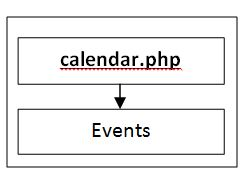
\includegraphics[width=0.60\textwidth]{images/calendar}
 \caption{Calendar Subsystem Diagram}
\end{figure}

\subsubsection{Assumptions}
The predinfined php structures were actually connected to the css calendar.


\subsubsection{Responsibilities}
The calendar allowed users to move around events on the calendar. Also, the oher responsibility was to display the events.


\subsubsection{Subsystem Interfaces}


\begin {table}[H]
\caption {Subsystem interfaces} 
\begin{center}
    \begin{tabular}{ | p{1cm} | p{6cm} | p{3cm} | p{3cm} |}
    \hline
    ID & Description & Inputs & Outputs \\ \hline
    \#1 & navigation & \pbox{3cm}{mouse click} & \pbox{3cm}{web address}  \\ \hline
    \end{tabular}
\end{center}
\end{table}

\subsection{Dashboard}
The dasboard allows students to sign up for simulation events.

\begin{figure}[h!]
	\centering
 	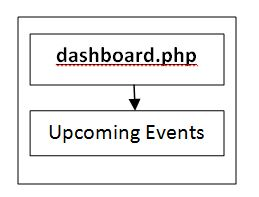
\includegraphics[width=0.60\textwidth]{images/dashboard}
 \caption{Dashboard Subsystem Diagram}
\end{figure}

\subsubsection{Assumptions}
No assumptions were made.

\subsubsection{Responsibilities}
The responsibility of the dashboard was to take user input. Also, to store the information into the database.


\subsubsection{Subsystem Interfaces}


\begin {table}[H]
\caption {Subsystem interfaces} 
\begin{center}
    \begin{tabular}{ | p{1cm} | p{6cm} | p{3cm} | p{3cm} |}
    \hline
    ID & Description & Inputs & Outputs \\ \hline
    \#1 & textfield & \pbox{3cm}{variable data} & \pbox{3cm}{true/false statement}  \\ \hline
    \end{tabular}
\end{center}
\end{table}

\subsection{Management}
The management allowed for administrators to manage their users.

\begin{figure}[h!]
	\centering
 	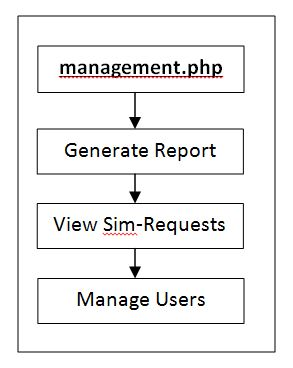
\includegraphics[width=0.60\textwidth]{images/management}
 \caption{Management Subsystem Diagram}
\end{figure}

\subsubsection{Assumptions}
The user has to be administrator to access the page.


\subsubsection{Responsibilities}
The responsibility of management was to manage users by deactivating or editing them. The editing allows for the administrator to change whether the user as student, gta, simulation tech, admin, and as well as some others. Another responsibility was to accept or reject simulation requests. Lastly, management generates a month report of the hours a user has worked.

\subsubsection{Subsystem Interfaces}


\begin {table}[H]
\caption {Subsystem interfaces} 
\begin{center}
    \begin{tabular}{ | p{1cm} | p{6cm} | p{3cm} | p{3cm} |}
    \hline
    ID & Description & Inputs & Outputs \\ \hline
    \#1 & buttons & \pbox{3cm}{mouse click} & \pbox{3cm}{action}  \\ \hline
    \#2 & POST & \pbox{3cm}{variable data} & \pbox{3cm}{N/A}  \\ \hline
    \#3 & naviagtion & \pbox{3cm}{mouse click} & \pbox{3cm}{web address}  \\ \hline
    \end{tabular}
\end{center}
\end{table}

\subsection{Inventory}
The inventory keeps tracks of inventory items.

\begin{figure}[h!]
	\centering
 	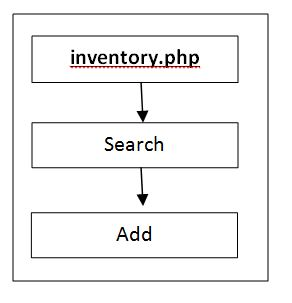
\includegraphics[width=0.60\textwidth]{images/inventory}
 \caption{Inventory Subsystem Diagram}
\end{figure}

\subsubsection{Assumptions}
No assumptions were made.


\subsubsection{Responsibilities}
The responsibility of the inventory was to display the inventory items from the database. Also, allows the user to edit, delete, and add inventory items.


\subsubsection{Subsystem Interfaces}


\begin {table}[H]
\caption {Subsystem interfaces} 
\begin{center}
    \begin{tabular}{ | p{1cm} | p{6cm} | p{3cm} | p{3cm} |}
    \hline
    ID & Description & Inputs & Outputs \\ \hline
    \#1 & buttons & \pbox{3cm}{mouse click} & \pbox{3cm}{action}  \\ \hline
    \#2 & textfield & \pbox{3cm}{variable data} & \pbox{3cm}{true/false statement}  \\ \hline
    \#3 & navigation & \pbox{3cm}{mouse click} & \pbox{3cm}{N/A}  \\ \hline
    \end{tabular}
\end{center}
\end{table}

